\documentclass[11pt]{article}
\usepackage{fullpage}
\usepackage{graphicx}
\usepackage{hyperref}
\begin{document}

\title{Homework 2 -- Monte Carlo Path Tracing}
\author{Gabe Fierro and Graham Tremper}
\date{\today}
\maketitle

\section{Introduction}

The code was compiled using GLM 0.9.4.1 on Mac OSX 10.7.4 and 10.8.2. To compile, run \verb`make` from
the \verb`PathTracing` directory. The test scenes are included in the \verb`testscenes` directory. The
compiled binary, \verb`raytracer` accepts 1 mandatory argument which is the path to the test scene, and
1 optional argument \verb`-f X`, where \verb`X` is the number of samples you wish to send at the scene.
For example

\begin{verbatim}
prompt> ./raytracer testscenes/cornell_box.test
prompt> ./raytracer -f 1000 testscenes/cornell_box.test
\end{verbatim}

If \verb`raytracer` is run without the optional \verb`-f` option, it enters an interactive mode. Pressing \verb`l`
will send a round of samples at the scene and render the result. Pressing \verb`f` will send 10000 samples
at the scene, and render after each result. Pressing \verb`s` will save the scene as a png file.

\section{Ray Tracing}

The project was built upon a basic ray tracer programmed for CS184, which supported rendering basic Phong models -- diffuse, specular and shiny surfaces. Triangle and sphere primitives are supported, and a KD-tree is used as an accelerating structure. This KD-tree had to be improved for this project, however, since the original implementation intersected many unnecessary bounding boxes. 

\section{Basic Implementation}

\subsection{Naïve Path Tracing}

We first implemented a simple path tracer that picked a random direction on the hemisphere at each bounce and a finite number of bounces. We terminated when hitting a emissive object, since we assume lights have no other reflective properties. This gave results with very high variance, and potential bias with the arbitrary depth limit. To speed up our renders, we used one of the instructional machines with the following specs: MacPro model 4,1, Quad-Core 2.26 GHz Intel Xeon (2 processors, 8 cores), 12-GB RAM

\subsection{Importance Sampling}

We implemented both macro and micro level importance sampling. For the macro level, we chose to shoot either a diffuse or specular ray based on the weight of the specular and diffuse weights for the primitive (We defined the weight as the averaged of the RGB values). At the micro level, we chose a ray direction using separate distributions for specular and diffuse.\\

Since diffuse rays distribute evenly in all directions, we important sampled according to the $\cos$ term in the rendering equation. This gave us the following distribution where $\theta$ is the angle between the surface normal and the selected ray direction.

\begin{equation}
	pdf(\theta) = \frac{\cos(\theta)}{\pi}
\end{equation}

For specular rays, we sampled in a hemisphere around the ideal reflection direction according to the specular BRDF. This gave us the following distribution, where $\alpha$ is the angle between the ideal reflection direction and the chosen ray and $n$ is the shininess.

\begin{equation}
	pdf(\alpha) = \frac{n+1}{2\pi}\cos^{n}(\alpha)
\end{equation}

\begin{figure}
  \begin{center}
    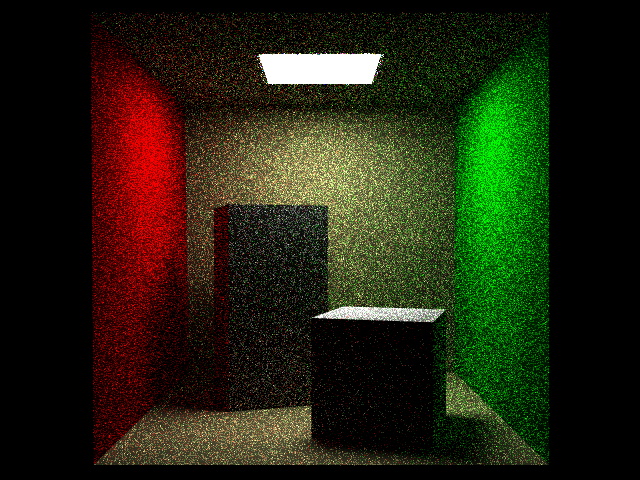
\includegraphics[width=.3\linewidth]{figs/impsample1cornell_low}
    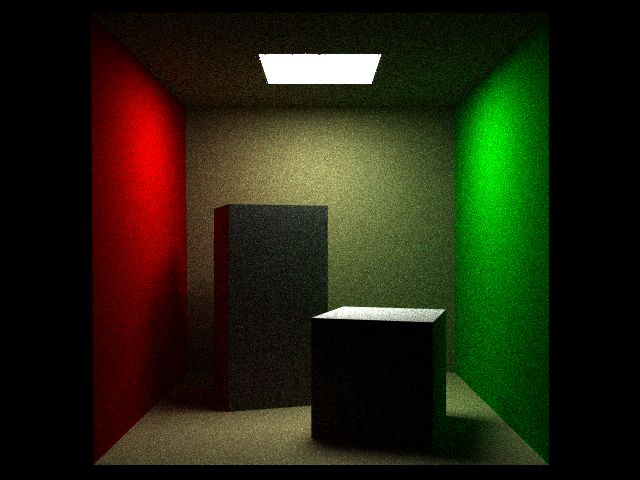
\includegraphics[width=.3\linewidth]{figs/impsample10cornell_low}
    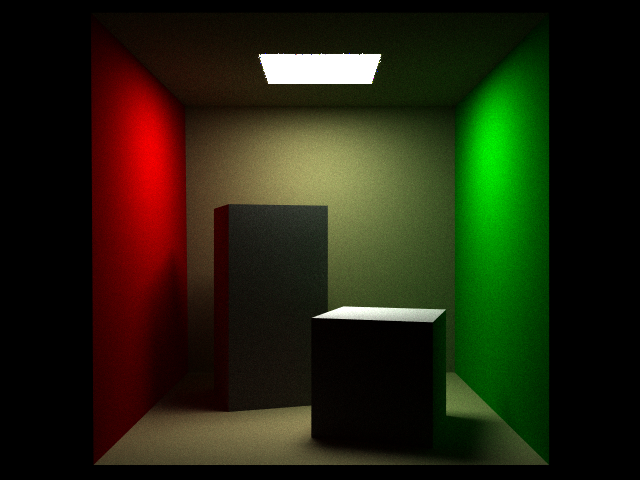
\includegraphics[width=.3\linewidth]{figs/impsample100cornell_low}
  \end{center}
  \caption{Importance Sampling with 16, 160 and 1600 samples per pixel. Direct lighting only on first bounce.}
\end{figure}

\begin{figure}
  \begin{center}
    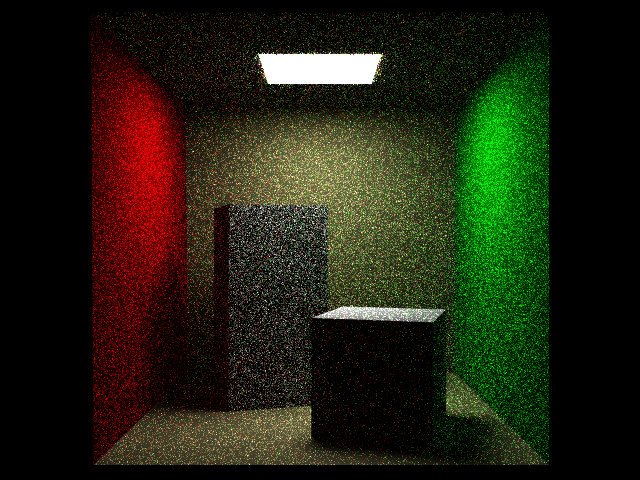
\includegraphics[width=.3\linewidth]{figs/noimpsample1cornell_low}
    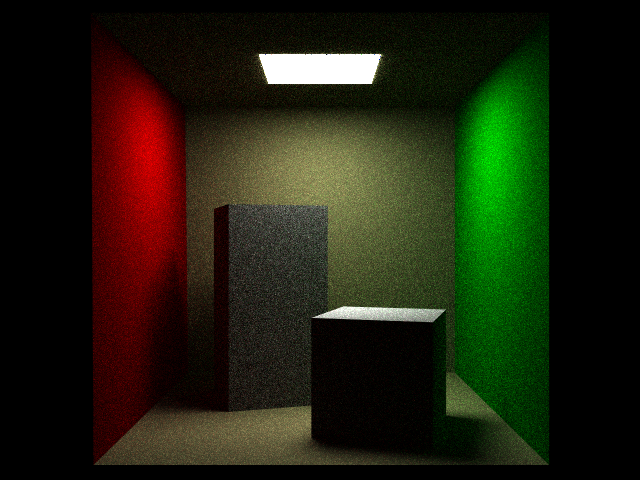
\includegraphics[width=.3\linewidth]{figs/noimpsample10cornell_low}
    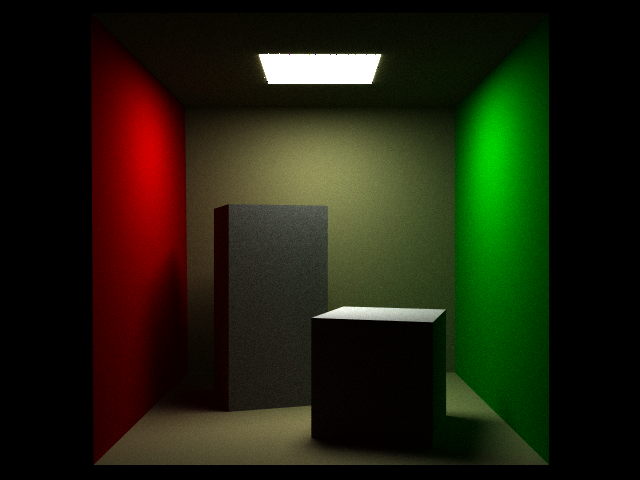
\includegraphics[width=.3\linewidth]{figs/noimpsample100cornell_low}
  \end{center}
  \caption{No Importance Sampling with 16, 160 and 1600 samples. Direct lighting only on first bounce.}
\end{figure}
\subsection{Direct Lighting}
Direct lightly allows some of the more important information to always be sampled, reducing the variance significantly. Run an initial direct lighting pass to capture all of single bounce lighting (Light paths in the form $L(S|D)E)$. We shot 12 shadow rays per sample, and used antialiasing to capture correct soft shadows. This only needs to be computed once, and the result is added to the final ``path traced'' image. We also tried shooting a single shadow ray per global illumination step to reduce variance, but found that this nearly doubled the sampling time without much reduction in variance. 

\begin{figure}
  \begin{center}
    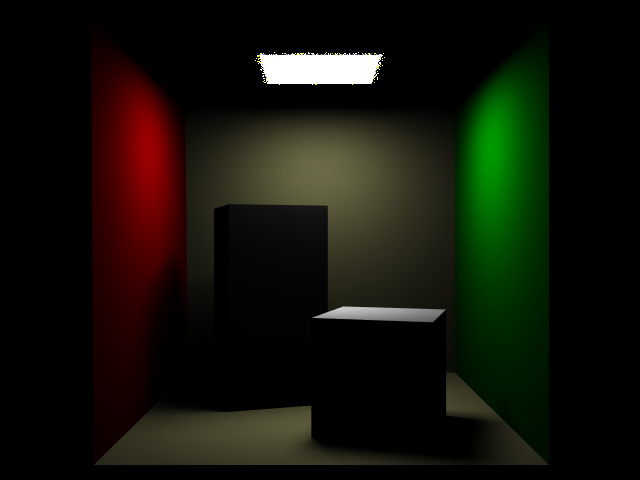
\includegraphics[width=.5\linewidth]{figs/direct_only_cornell}
  \end{center}
  \caption{Direct lighting only}
\end{figure}

\begin{figure}
  \begin{center}
  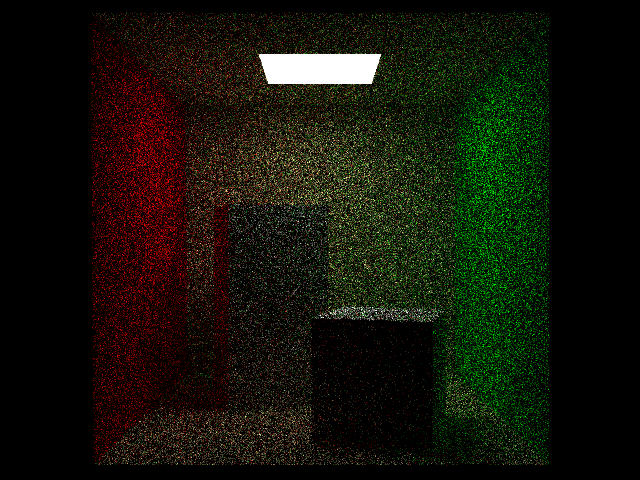
\includegraphics[width=.4\linewidth]{figs/indirect_only_1sample}
  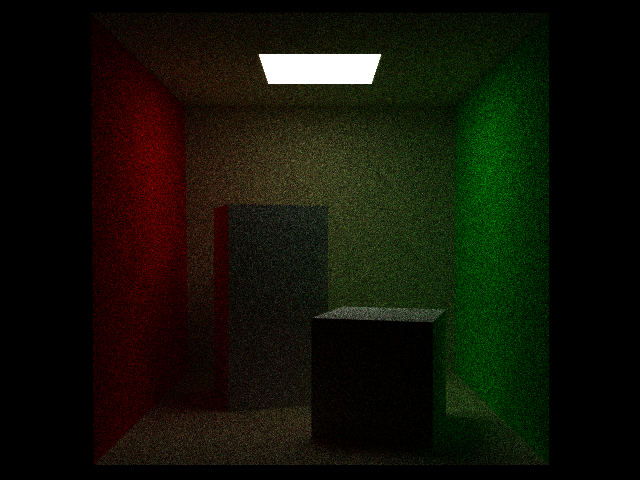
\includegraphics[width=.4\linewidth]{figs/indirect_only_10sample}
  \end{center}
  \caption{Indirect lighting only, with 1 and 10 samples}
\end{figure}

\section{Extra Features}

\subsection{Russian Roulette}
Russian roulette allows for a ray termination scheme without introducing bias in the final picture that techniques such as a depth limit will introduce. We stored a weight associated with each ray that represented how much that color will contribute to the final image. When this weight falls bellow $0.01$, we kill $90\%$ of the rays and appropriately weight the surviving rays. We found this ratio didn't negatively effect performance or the variance.

\subsection{Soft Shadows}
We implemented soft shadows by using stratified sampling on the area lights. This was non-trivial, since we used triangle shaped emissive surfaces. In order to correctly stratify the triangle, we divided the triangle into six sections of equal area. This was done by finding the centroid of the triangle, and creating 6 new triangles as shown in the figure below. This process could be applied recursively for further stratification, but we found this unnecessary for the images we generated.

\begin{figure}
	\begin{center}
		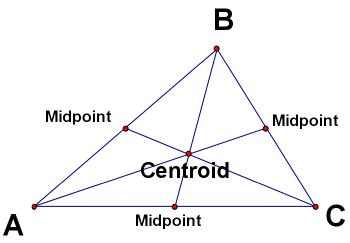
\includegraphics[width=.5\linewidth]{figs/centroid}
		\caption{Each of these six triangles has the same area.}
	\end{center}
\end{figure}

For the global illumination, we achieved area lighting by simply having the lights be real objects in the scene. We assumed lights had no other reflective properties, so rays could always be terminated when one was hit. We also tried sampling the area light with a single shadow ray for each path tracer bounce, but had a large increase in compute time without much reduction in variance, so we omitted it.

\subsection{Anti-aliasing}

We implemented anti-aliasing by using a jittered sampling of the pixel for each sample. To reduce variance, we stratified the pixel based on the level of antialiasing to reduce variance. This works especially well with path tracing since we need to sample each pixel multiple times anyway. For most of our pictures, we used a 4x4 grid with 16 samples per pixel per iteration. 

\section{Results}

\begin{figure}
	\begin{center}
		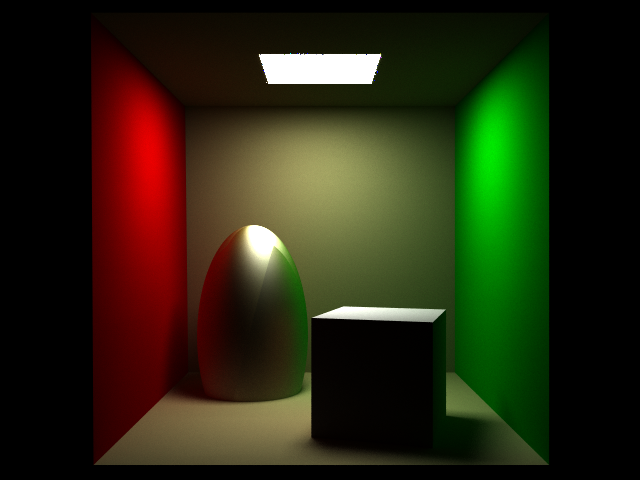
\includegraphics[width=.5\linewidth]{figs/specular_ellipse_1000samples}
		\caption{1000 Samples, with importance sampling and antialiasing. Note the specular highlights
		on the ellipse and color bleeding from the walls.}
	\end{center}
\end{figure}
\begin{figure}
	\begin{center}
		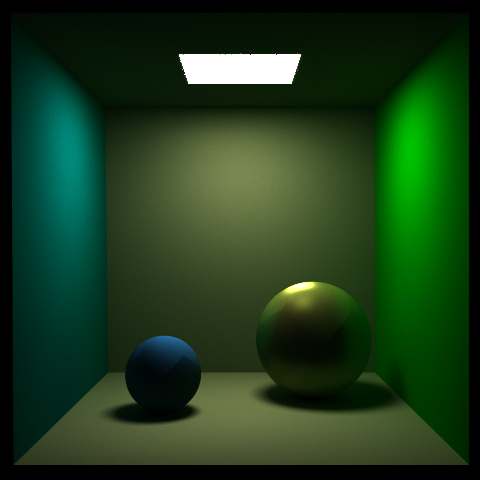
\includegraphics[width=.5\linewidth]{figs/2spheres_1000samples}
		\caption{1000 Samples, with importance sampling and antialiasing. Blue diffuse and yellow mirror spheres.}
	\end{center}
\end{figure}



\end{document}
